\chapter{La recommendation}

\section{Introduzione}

Come fa \textit{Spotify} a sapere quale canzone potresti voler ascoltare? E come fa \textit{Netflix} a suggerirti la prossima serie da guardare? Questo è possibile grazie al modello di \textit{recommendation} basato su \textit{machine learning} che analizza cosa piace all'utente e gli propone contenuti su misura. Di solito si utilizzano due tipi principali di raccomandazioni:

\begin{itemize}
    \item per la \textit{home page}: i consigli sono personalizzati per un utente in base ai suoi interessi. Ogni utente vede consigli diversi
    \item su articoli correlati: sono consigli simili a un di un articolo specifico. Per esempio in Google Play, gli utenti che visualizzano la pagina di un'app di matematica potrebbero vedere anche un riquadro con app correlate, come altre app di matematica o di scienze
\end{itemize}

Un sistema di \textit{recommendation} aiuta gli utenti a scoprire contenuti interessanti all'interno di un'enorme quantità di dati. Per esempio su YouTube ci sono miliardi di video, con nuovi contenuti che vengono aggiunti ogni giorno. Come può un utente trovare qualcosa di nuovo che valga la pena guardare o provare? La ricerca manuale è un'opzione. Tuttavia, un motore di raccomandazione è in grado di suggerire contenuti che magari l'utente non avrebbe mai pensato di cercare da solo. Basti sapere che, secondo quanto dice \textit{Google}:

\begin{itemize}
    \item il 40\% delle app installate dal \textit{Google Play} derivano da raccomandazioni
    \item il 60\% del tempo di visualizzazione su \textit{YouTube} proviene dalle raccomandazioni
\end{itemize}


\subsubsection{Terminologia}
Ci sono alcuni termini da introdurre:

\begin{itemize}
    \item \textit{item}: sono gli elementi/entità consigliate dal sistema. Su \textit{Spotify} sono le canzoni, su \textit{Amazon} sono i prodotti, su \textit{Intragram} sono i \textit{post}
    \item \textit{query}: sono le informazioni utilizzate da un sistema per fornire consigli. Le \textit{query} possono essere una combinazione di informazioni dell'utente (e.g. ID, elementi con i quali ha interagito in passato etc.) e contesto aggiuntivo (e.g. ora del giorno, per quanto tempo ha osservato quel prodotto o quell'episodio etc.)
\end{itemize}

I passaggi tipici che ti utilizzano sono: 

\begin{enumerate}
    \item generazione dei candidati: il sistema parte da un corpus di \textit{item}, potenzialmente enorme, e ne estrae un sottoinsieme molto più piccolo di candidati
    \item calcolo dello \textit{score}: un altro modello, più preciso del primo dato che lavora su una quantità molto minore di dati, assegna un punteggio ai candidati
    \item \textit{re-ranking}: i candidati vengono ordinati per lo score ricevuto considerando eventuali ulteriori vincoli (e.g. rimuovendo contenuti che l'utente ha segnalato come non graditi, oppure aumentare il punteggio di contenuti più recenti). Il riordinamento può garantire maggiore varietà, attualità e imparzialità.
\end{enumerate}

\section{Generazione dei candidati}\label{generazione_dei_candidati}

\subsubsection{Embedding}

Gli \textit{item} e le \textit{query} vengono mappati su  vettore di \textit{embedding} in uno spazio comune $E = \mathbb{R}^k$. Normalmente lo spazio di \textit{embedding} ha una dimensione molto più piccola rispetto alla grandezza del corpus e cattura alcune strutture latenti dell'insieme di \textit{item} o \textit{query}. Gli elementi tra loro simili finiscono per essere vicini nello spazio di \textit{embedding}. Il concetto di ``vicinanza" è definito da una misura di similarità.
 
\subsubsection{Calcolo della similarità}

Una misura di similarità è una funzione $s: E \times E \to \mathbb{R}$ che prende in input una coppia di vettori di \textit{embedding} e restituisce un valore scalare che ne misura la similarità. Gli \textit{embedding} possono essere utilizzati per la generazione dei candidati come segue: dato un vettore di \textit{embedding} per una query $q \in E$, il sistema cerca gli \textit{embedding} degli elementi $x \in E$ che sono vicini a $q$, ossia, gli \textit{embedding} con una similarità elevata.

Per determinare il grado di similarità, la maggior parte dei sistemi di \textit{recommendation} si basa su una o più delle seguenti misure:

\begin{itemize}
    \item coseno: semplicemente il coseno dell'angolo tra i due vettori $s(q, x) = cos(q, x)$
    \item prodotto scalare: è dato da: $s(q, x) = \langle q, x \rangle = \sum\limits_{i=1}^{d} q_i x_i$. È anche dato da $s(q, x) = \|x\| \|q\| \cos(q, x)$ che corrisponde al coseno dell'angolo moltiplicato per il prodotto delle norme. Pertanto, se gli \textit{embedding} sono normalizzati, il prodotto scalare e il coseno coincidono    
    \item distanza euclidea: questa è la distanza usuale nello spazio euclideo $s(q, x) = \|q - x\| = \left[ \sum\limits_{i=1}^{d} (q_i - x_i)^2 \right]^{\frac{1}{2}}$. Una distanza minore indica una similarità maggiore. Da notare che, quando gli \textit{embedding} sono normalizzati, la distanza euclidea al quadrato coincide con il prodotto scalare (e il coseno) fino a una costante, poiché in quel caso $\frac{1}{2} \|q - x\|^2 = 1 - \langle q, x \rangle$
\end{itemize}


\begin{figure}[H]
    \centering
    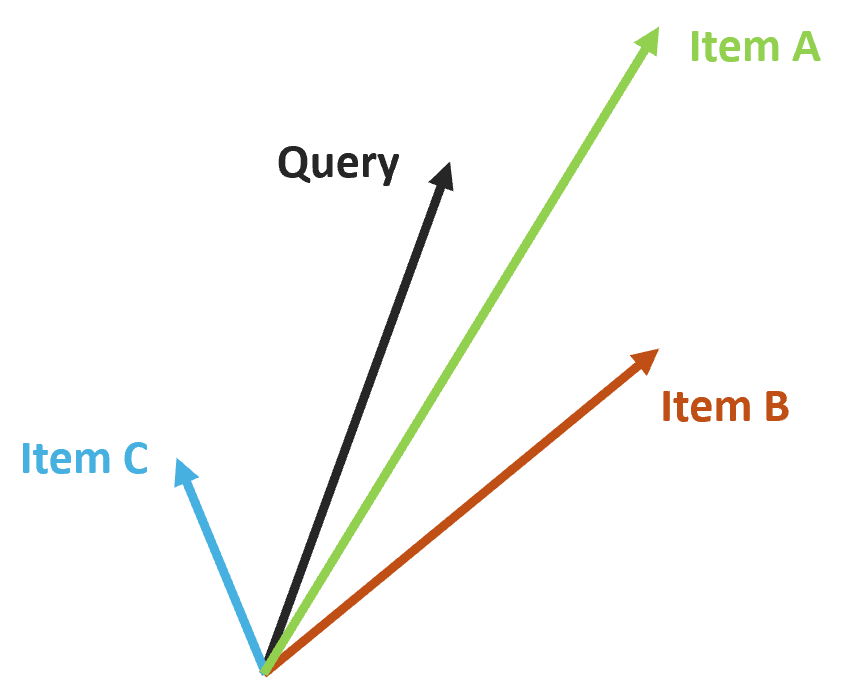
\includegraphics[scale=0.8]{figures/embedding.PNG}
    \caption{Il vettore nero illustra l'\textit{embedding} della query. Gli altri tre vettori di \textit{embedding} (\textit{Item A}, \textit{Item B}, \textit{Item C}) rappresentano gli \text{item} candidati. A seconda della misura di similarità utilizzata, la classifica degli elementi può essere diversa}
    \label{fig:embedding}
\end{figure}

Rispetto al coseno, la similarità del prodotto scalare è sensibile alla norma dell'\textit{embedding}. Cioè, maggiore è la norma di un \textit{embedding}, maggiore sarà la similarità e più è probabile che l'\textit{item} venga raccomandato. Questo può influenzare le raccomandazioni nei seguenti modi:

\begin{itemize}
    \item gli elementi che appaiono molto frequentemente nel \textit{training set} (ad esempio, le top canzoni italiane del momento su \textit{Spotify}) tendono ad avere \textit{embedding} con norme grandi. Se è desiderabile catturare informazioni sulla popolarità, allora si dovrebbe preferire il prodotto scalare. Tuttavia, se non si presta attenzione, gli elementi popolari potrebbero finire per dominare le raccomandazioni. In pratica, si possono utilizzare altre varianti delle misure di similarità che pongono meno enfasi sulla norma dell'\textit{item}. Ad esempio, definire $s(q, x) = \|q\|^{\alpha} \|x\|^{\alpha} \cos(q, x)$ per qualche $\alpha \in (0,1)$
    \item Gli elementi che appaiono molto raramente potrebbero non essere aggiornati frequentemente durante l'addestramento. Di conseguenza, se vengono inizializzati con una norma elevata, il sistema potrebbe raccomandare elementi rari invece di quelli più rilevanti. Per evitare questo problema, prestare attenzione all'inizializzazione degli \textit{embedding} e utilizzare una regolarizzazione appropriata
\end{itemize}


Le due tecniche più comuni per la generazione dei candidati sono:

\begin{itemize}
    \item \textit{content-based filtering}
    \item \textit{collaborative filtering}
\end{itemize}
  
\section{Content-based filtering}
Il \textit{content-based filtering} utilizza la similarità tra gli oggetti per raccomandare elementi simili a quelli che l'utente apprezza o ha apprezzato. Ad esempio, se l'utente $A$ guarda due film \textit{fantasy}, il sistema può raccomandargli altri film dello stesso genere.

L'idea è che se ad un utente è piaciuto un certo \textit{item} con certe caratteristiche, il sistema proporrà altri \textit{item} simili per contenuto.

Per prima cosa si crea un profilo degli \textit{item}, cioè viene rappresentato tramite un insieme di caratteristiche (\textit{feature}). Per un film, per esempio, si possono utilizzare il/i generi, gli attori principali, l'anno di uscita, la durata etc.

Dopodiché si costruisce un profilo dell'utente analizzando gli oggetti che ha valutato positivamente. Il profilo rappresenta una media delle caratteristiche degli oggetti preferiti.

Si confronta il profilo dell'utente con gli \textit{item} non ancora visti usando una metrica di similarità (es. coseno, distanza euclidea~\ref{generazione_dei_candidati}).

vengono raccomandati gli \textit{item} più simili al profilo dell'utente.

\subsubsection{Esempio}

Si supponga che all'utente $A$ siano piaciuti due film:

\begin{itemize}
    \item \textit{Matrix} i cui generi sono \textit{Azione} e \textit{Fantascienza}
    \item \textit{Inception} i cui generi sono \textit{Azione}, \textit{Fantascienza} e \textit{Thriller}
\end{itemize}

Si crea il profilo dell'utente con la media delle caratteristiche: 

\begin{itemize}
    \item \textit{Azione} $= 1$
    \item \textit{Fantascienza} $= 1$
    \item \textit{Thriller} $= 0.5$
\end{itemize}

Poi si selezionano altri film dal catalogo, ad esempio:

\begin{itemize}
    \item \textit{Interstellar} i cui generi sono \textit{Fantascienza} e \textit{Drammatico}
    \item \textit{John Wick} il cui genere è \textit{Azione}
\end{itemize}

\begin{figure}[H]
    \centering
    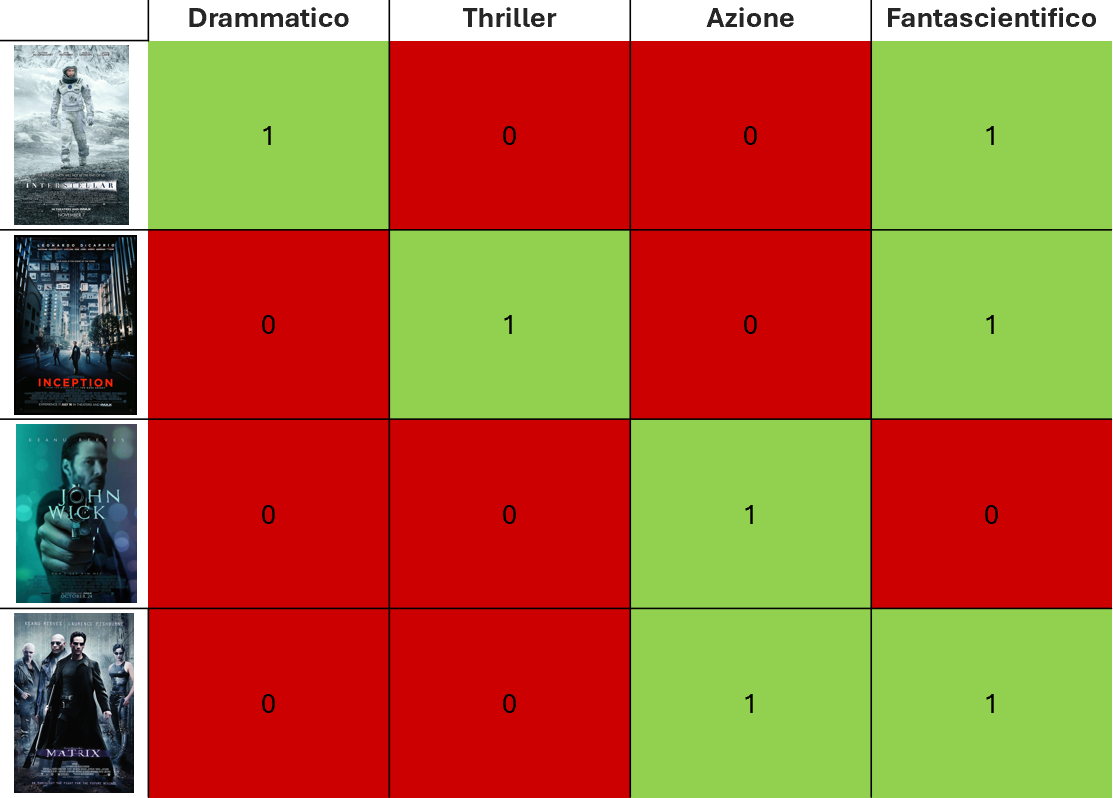
\includegraphics[scale=0.5]{figures/content_based_filtering.PNG}
    \caption{La figura mostra i vettori delle caratteristiche dei film (in questo caso il genere) per i film in esempio. Se il film appartiene ad uno specifico genere viene posto il valore $1$, altrimenti $0$}
    \label{fig:item_vector}
\end{figure}

Si creano vettori per i film considerando tutti i generi analizzati fino ad ora e si calcola la similarità con il profilo dell'utente. Si ottiene, utilizzando per esempio la similarità coseno, un valore di $0.47$ per $Interstellar$ e di $0.67$ per \textit{John Wick}, quindi quest'ultimo viene raccomandato prima di \textit{Interstellar}, perché è più simile al profilo dell'utente.


\subsubsection{Vantaggi e svantaggi}

I vantaggi di quest'approccio sono:
\begin{itemize}
    \item il modello non ha bisogno di dati su altri utenti, poiché le raccomandazioni sono specifiche per questo utente. questo lo rende più facile da scalare a un grande numero di utenti
    \item il modello può catturare gli interessi specifici di un utente e può raccomandare \textit{item} di nicchia che interessano a pochissimi altri utenti
\end{itemize}

Gli svantaggi di quest'approccio sono:
\begin{itemize}
    \item poiché la rappresentazione delle caratteristiche degli oggetti è in parte progettata manualmente, questa tecnica richiede molta conoscenza del dominio. Il modello può essere solo quindi valido quanto le caratteristiche progettate manualmente
    \item il modello può fare raccomandazioni solo basate sugli interessi esistenti dell'utente. In altre parole, ha una capacità limitata di espandere gli interessi dell'utente
\end{itemize}

\section{Collaborative filtering}

Per affrontare alcune delle limitazioni del \textit{content-base filtering}, il \textit{collaborative filtering} utilizza simultaneamente le somiglianze tra utenti e \textit{item} per fornire raccomandazioni. I modelli possono raccomandare un \textit{item} all'utente $A$ in base agli interessi di un utente simile $B$ anche se $A$ non ha mai visto \textit{item} simili. Inoltre, gli \textit{embedding} possono essere appresi automaticamente, senza dover progettare manualmente le caratteristiche.

Si consideri un sistema di raccomandazione di film in cui i dati di addestramento consistono in una matrice di feedback in cui:

\begin{itemize}
    \item Ogni riga rappresenta un utente.
    \item Ogni colonna rappresenta un \textit{item} (un film).
    \item Il feedback sui film rientra in una delle due categorie:
    \begin{itemize}
        \item esplicito: gli utenti specificano quanto gli è piaciuto un determinato film fornendo una valutazione numerica.
        \item implicito: se un utente guarda un film, il sistema deduce che l'utente è interessato.
    \end{itemize}
\end{itemize}

Per semplificare, si supponga che la matrice di feedback sia binaria; cioè, un valore di $1$ indica interesse per il film.

Quando un utente visita la homepage, il sistema dovrebbe raccomandare film basati su:

\begin{enumerate}
    \item somiglianza con i film che l'utente ha apprezzato in passato
    \item film che utenti simili hanno apprezzato
\end{enumerate}

\subsubsection{1D embedding}

Si assegna a ciascun film uno scalare in $[-1, 1]$ che descriva se il film è destinato a bambini (valori negativi) o ad adulti (valori positivi). Allo stesso modo, per ciascun utente si assegna uno scalare in $[-1, 1]$ che descriva il suo interesse per i film per bambini o per adulti. Il prodotto dell'\textit{embedding} del film e dell'\textit{embedding} dell'utente dovrebbe essere più alto (vicino a 1) per i film che dovrebbero piacere all'utente.

\begin{figure}[H]
    \centering
    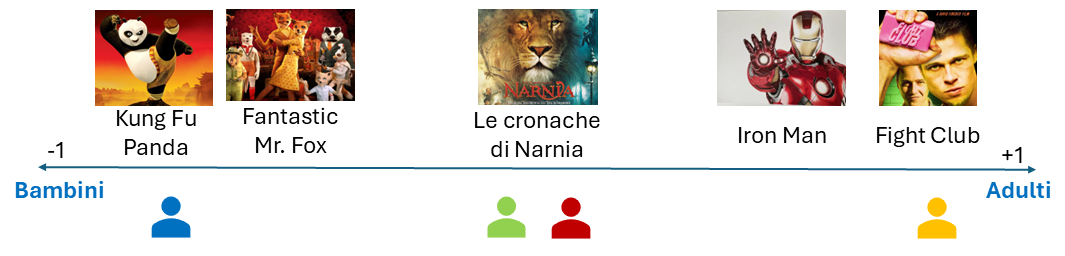
\includegraphics[scale=0.4]{figures/collaborative_filtering/embeddings.PNG}
    \caption{Rappresentazione su un asse 1D delle posizioni di utenti e film rispetto allo scalare assegnato nell'intervallo $[-1, 1]$}
    \label{fig:embeddings}
\end{figure}

Nella seguente matrice, ogni segno di spunta identifica un film che un determinato utente ha guardato. Il terzo e il quarto utente hanno preferenze evidenti per questa caratteristica: il terzo utente preferisce i film per bambini, mentre il quarto preferisce i film per adulti. Ciò non vale invece per il primo e del secondo utente.

\begin{figure}[H]
    \centering
    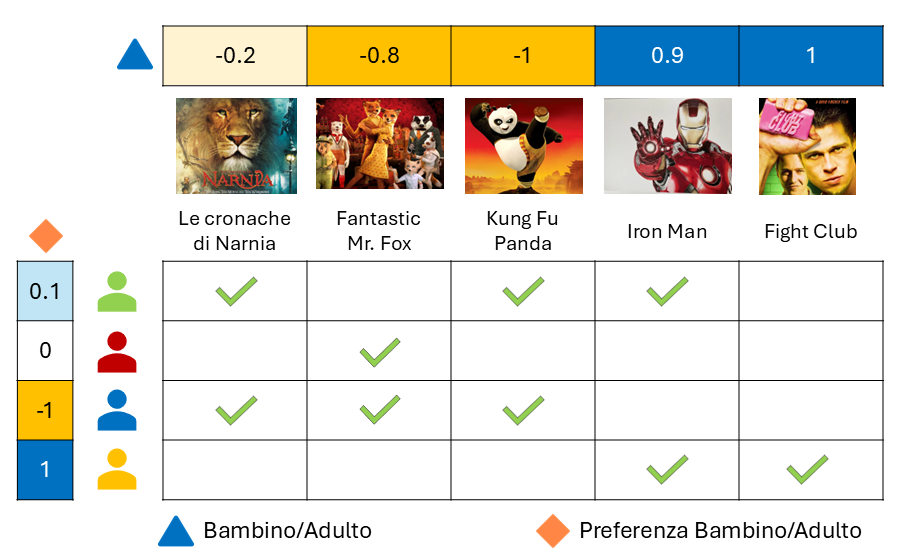
\includegraphics[scale=0.5]{figures/collaborative_filtering/1D_matrix.PNG}
    \caption{matrice che mostra i film guardati dagli utenti, le categorie dei film e le preferenze degli utenti}
    \label{fig:1D_matrix}
\end{figure}

\subsubsection{2D embedding}

Una sola caratteristica non è sufficiente a spiegare le preferenze di tutti gli utenti. Per superare questo problema, si utilizza una seconda caratteristica: il grado in cui ogni film è un \textit{blockbuster} (film molto popolare e di grande successo al botteghino) o un film d'autore. Con una seconda caratteristica, ora si può rappresentare ogni film con il seguente \textit{embedding} bidimensionale:

\begin{figure}[H]
    \centering
    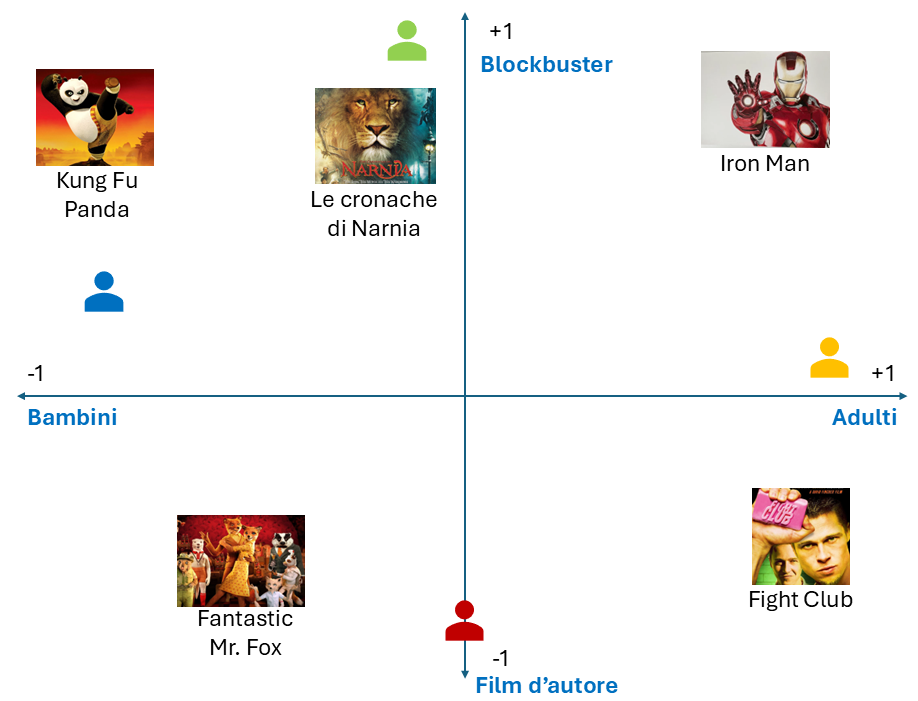
\includegraphics[scale=0.4]{figures/collaborative_filtering/axes.PNG}
    \caption{gli assi mostrano, per ciascuna caratteristica, la posizione dei film e le preferenze degli utenti}
    \label{fig:embedding_axes}
\end{figure}

Nel grafico sono rappresentati sia gli elementi che gli utenti nello stesso spazio di \textit{embedding}. Questo perché si può pensare allo spazio di \textit{embedding} come a una rappresentazione astratta comune sia agli \textit{item} che agli utenti, in cui si può misurare la similarità.

\begin{figure}[H]
    \centering
    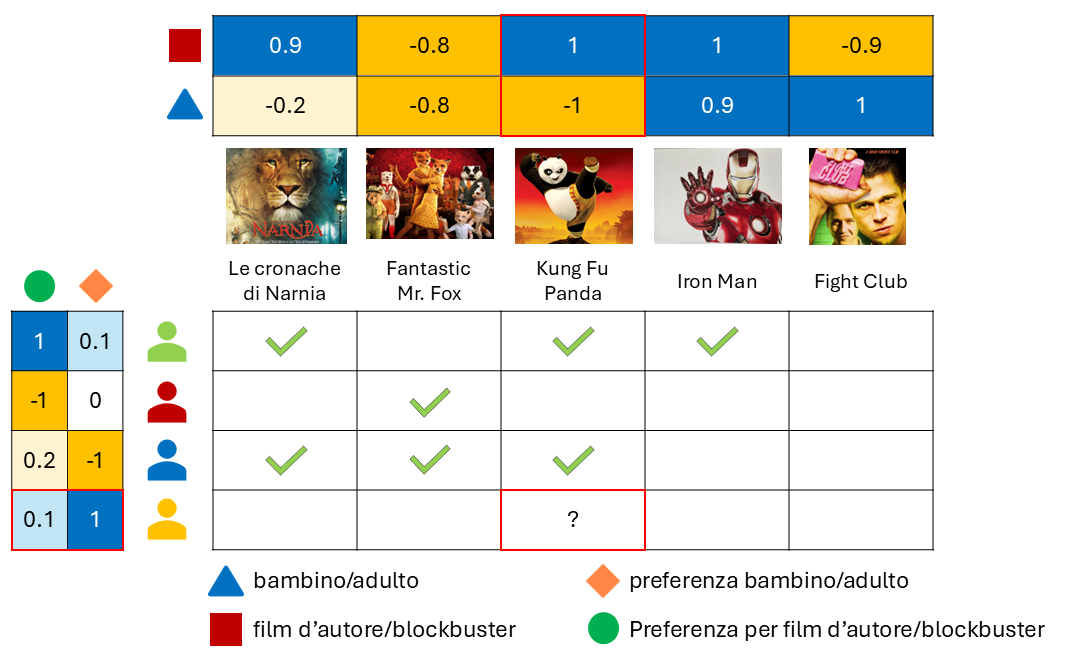
\includegraphics[scale=0.4]{figures/collaborative_filtering/2D_matrix.PNG}
    \caption{matrice che mostra i film guardati dagli utenti, le categorie dei film e le preferenze degli utenti estese}
    \label{fig:2D_matrix}
\end{figure}

L'obbiettivo è che per ogni coppia (utente, \textit{item}) il prodotto scalare dell'\textit{embedding} dell'utente e dell'\textit{embedding} dell'\textit{item} fosse vicino a $1$ quando l'utente ha guardato il film e a $0$ in caso contrario.

I modelli apprendono automaticamente un vettore di \textit{embedding} per ciascun utente che spieghi al meglio le sue preferenze. Di conseguenza, gli \textit{embedding} di utenti con gusti simili risulteranno vicini tra loro. Allo stesso modo il modello apprende gli \textit{embedding} dei film in modo da spiegare al meglio la matrice di feedback. Anche in questo caso, gli \textit{embedding} dei film apprezzati da utenti simili saranno vicini nello spazio degli embedding.

\subsubsection{Vantaggi e svantaggi}

I vantaggi di quest'approccio sono:

\begin{itemize}
  \item non è necessaria conoscenza del dominio: gli embedding vengono appresi automaticamente
  \item serendipità: anche se il modello non sa che l'utente è interessato a un determinato \textit{item} potrebbe comunque raccomandarlo perché utenti simili sono interessati a quell'\textit{item}
  \item ottimo punto di partenza: il sistema ha bisogno solo della matrice di feedback, e non di informazioni contestuali, per addestrare un modello
\end{itemize}

Gli svantaggi di quest'approccio sono:

\begin{itemize}
  \item non si può gestire \textit{item} nuovi: se un oggetto non è stato visto durante l'addestramento, il sistema non può creare un \textit{embedding} per esso. Questo problema è noto come \textit{cold-start}. Tuttavia, esistono tecniche che possono affrontare in parte questo problema: 

  \begin{itemize}
    \item proiezione: dato un nuovo \textit{item} $i_0$ non visto durante l'addestramento, se il sistema ha alcune interazioni con utenti, può facilmente calcolare un \textit{embedding} per quell'\textit{item} senza riaddestrare l'intero modello. Basta risolvere la seguente equazione (o la sua versione pesata):

    \[
    \min_x \sum_{i}(r_{ui} - x^T u_i)^2
    \]

    Gli \textit{embedding} dell'utente vengono mantenuti fissi, e il sistema risolve per ottenere l'\textit{embedding} dell'\textit{item}. Lo stesso approccio può essere utilizzato per un nuovo utente.
    \item euristiche: se il sistema non ha interazioni, può approssimare l'\textit{embedding} di un \textit{item} facendo la media degli \textit{embedding} di \textit{item} appartenenti alla stessa categoria
  \end{itemize}

  \item difficoltà nell'includere caratteristiche aggiuntive per \textit{query}/\textit{item}: le caratteristiche aggiuntive (\textit{side features}) sono tutte quelle informazioni oltre all'ID della query o dell'\text{item}. Per esempio, per i film, le caratteristiche possono includere il paese o l'età. Includere queste caratteristiche migliora la qualità del modello

  Per generalizzare WALS, si può estendere la matrice di input includendo le caratteristiche, definendo una matrice a blocchi $\tilde{R}$:

  \[
  \tilde{R} = \begin{bmatrix}
  R & U_f \\
  I_f & 0
  \end{bmatrix}
  \]

  dove:
  \begin{itemize}
    \item $R$ è la matrice di feedback tra utenti e \textit{item};
    \item $U_f$ è una codifica multi-hot delle feature degli utenti (per esempio età, paese, genere);
    \item $I_f$ è una codifica multi-hot delle feature degli \textit{item} (per esempio categoria, lingua, creatore);
    \item $0$ è una matrice di zeri, che rappresenta l'assenza di interazioni dirette tra le feature utente e quelle degli \textit{item}.
  \end{itemize}
\end{itemize}

\section{Matrix Factorization}

In questa parte viene data una breve introduzione alla tecnica della \textit{Matrix Factorization} dato che molti degli algoritmi presentati la utilizzano come base dei propri algoritmi.

La \textit{Matrix Factorization} è una tecnica utilizzata per rappresentare una matrice come prodotto di due o più matrici. Consente di estrarre strutture latenti dai dati, rendendo possibile la scoperta di relazioni implicite tra entità \cite{MC}.

Questa tecnica è alla base di molte applicazioni in ambiti diversi, tra cui l'elaborazione di segnali, la compressione dei dati, la visione artificiale e, in particolare, i sistemi di \textit{recommendation}.

Formalmente, data una matrice $R \in \mathbb{R}^{m \times n}$, la fattorizzazione mira a trovare due matrici $W \in \mathbb{R}^{m \times k}$ e $H \in \mathbb{R}^{n \times k}$ tali che:
\[
R \approx WH^T
\]
dove 
\begin{itemize}
    \item le righe di $W$ corrispondono agli \textit{embedding} degli utenti
    \item le righe di $H$ corrispondono agli \textit{embedding} degli \textit{item}
    \item $k \ll \min(m,n)$ è il rango latente scelto
\end{itemize}

\begin{figure}[H]
    \centering
    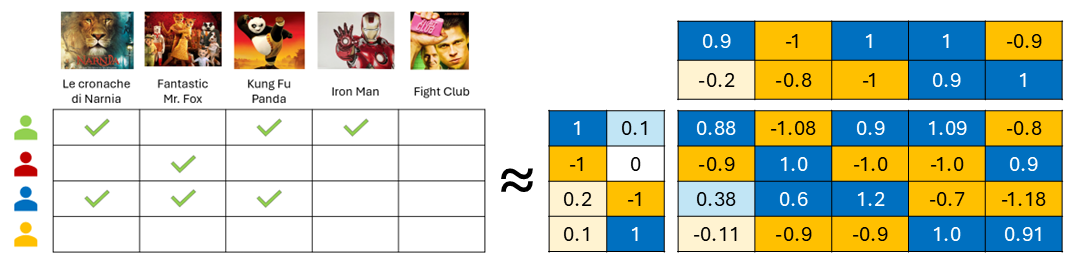
\includegraphics[scale=0.5]{figures/matrix_factorization.PNG}
    \caption{rappresentazione della matrice $R$ come prodotto delle due matrici $W$ e $H$}
    \label{fig:matrix_factorization}
\end{figure}

Questa approssimazione riduce la dimensionalità dei dati, semplifica il modello e cattura le relazioni principali presenti nella matrice originaria.

Un celebre esempio dell'efficacia di questa tecnica nei sistemi di \textit{recommendation} è il \textit{Netflix Prize} del 2006. Il team vincente la utilizzò per migliorare le previsioni di rating del 10\% rispetto al sistema originario di Netflix \cite{TheNP}.

I principali vantaggi nel suo utilizzo sono la scalabilità, poiché i modelli sono efficienti da memorizzare e computare, e la capacità di generalizzazione, in quanto riescono a catturare relazioni latenti non esplicitamente osservate. Tuttavia, esistono anche alcuni limiti, tra cui il problema della \textit{cold start}, che rende difficile raccomandare per nuovi utenti o nuovi item, e la sparsità, che può portare a una una bassa qualità delle raccomandazioni\cite{SVD_analysis}.

Pur con alcune limitazioni, essa costituisce la base per molti degli algoritmi di \textit{recommendation} più efficaci oggi in uso, ed è spesso integrata con approcci più complessi, come i modelli Deep Learning o i grafi.


\section{Sistemi ibridi}